\documentclass{llncs}
	\usepackage{mathtools}
	\usepackage{amsmath}
	\usepackage{algorithm2e}
	\usepackage{graphicx}
	\usepackage{hyperref}

\makeatletter
\renewcommand{\@algocf@capt@plain}{above} 
\makeatother

\begin{document}

\title{Simulating International Energy Security}
	\author{David Masad}
	\institute{Department of Computational Social Science\\George Mason University\\Fairfax, VA}
	\maketitle


\begin{abstract}
Energy security is placed at risk by exogenous supply shocks, in particular political crises and conflicts that disrupt resource extraction and transportation. In this paper, a computational model of the security of international crude oil supplies is described, and its output analyzed. The model consists of country agents, linked geographically and by a data-derived oil trade network. Countries stochastically experience crises, with probabilities and durations drawn randomly from data-fitted distributions. The effect of these crises on secure oil supplies is measured globally and by country, and the effect of conflict contagion and spare production capacity are also estimated. The model indicates that Russia, Eastern Europe, and much of the Global South are at the greatest risk of supply shocks, while American producers are at greatest risk of demand shocks. It estimates that conflict contagion decreases energy security slightly, while spare capacity has minimal effect. 
\end{abstract}

\section{Introduction}

Energy security is defined by the International Energy Agency as ``the uninterrupted availability of energy sources at an affordable price''\cite{iea_2013}. As the world's energy demand continues to expand, energy security is becoming increasingly critical not just to developed countries but to developing ones as well \cite{yergin_2006}. Much of the previous formal analysis of energy security has taken a portfolio-based approach, examining both the short-term risks\cite{wu_2009,jewell_2011} and long-term energy and environmental policy \cite{stirling_2010,skea_2010,jacobson_2009}. However, these approaches tend to aggregate political risk into a single indicator, and do not incorporate the complexity that characterizes international political in general, and conflict in particular \cite{cederman_1997,geller_2011}. In fact, oil supply shocks are often caused by domestic or international conflicts involving oil producers \cite{hamilton_2003}. While the macroeconomic effects of oil shocks may be small \cite{kilian_2008}, the price of oil is only an indirect measure of energy security. If a substantial volume of oil cannot be extracted or exported, and hence is unavailable for consumption, this poses an energy security risk regardless of the benchmark price. 

In this paper, I present a novel model linking energy security with political instability. At the core of the model is the supply and demand for crude oil at the country level. Supply and demand are placed at risk when countries experience crises and conflicts. The model operates on the meso timescale, of months and years rather than days or decades.  It produces country-level and global time-series of oil security indicators with each iteration. By running multiple iterations with different parameters, I generate notional near-future scenarios of changes in international energy security. By incrementally enabling the possibility of conflict contagion, and of rapid increases of production to counterbalance supply shocks, I can estimate their impact on international energy security. 

In the remainder of the paper, I describe the model in more detail, as well as its input data sources. I use the model to conduct several experiment and describe the output. Finally, I discuss my conclusions, both regarding international energy security and the challenges and opportunities of this type of modeling.

\section{Model}

\subsection{Model Description}

The model consists of countries, each of which has a set supply of and demand for crude oil\footnote{Full model code is available at \url{https://github.com/dmasad/riskworld}}. Countries are linked geographically to their neighbors, and by a network of export-import relationships. Each monthly tick of the model, some countries enter crisis at random with probability based on their political instability. Crisis duration is randomly drawn from a power law distribution. The exports and imports of countries in crisis are considered \emph{at risk}. At the end of each tick, the model measures several indicators of oil security. The Overall Ratio is the global ratio of secure demand to secure supply; a high ratio indicates a higher likelihood of a global supply shock, while a low ratio indicates a higher likelihood of a global demand shock. For each country, the model computes the ratio of total demand to secure (not at risk) supply (the Supply Ratio). The higher this ratio is, the more likely the country is to experience a supply shock. The model also computes the fraction of each country's total exports are going to countries not in crisis (Demand Ratio), estimating the risk of a demand shock.

If \textbf{Contagion} is enabled, when a country enters crisis it may trigger crises in neighboring countries based on their own instability. If \textbf{Assistance} is enabled, oil exporters may utilize their spare capacity and increase their production to balance a loss of secure oil by a major import partner, increasing the supply of oil to all of their trading partners.

\subsection{Data Sources}
The network of oil imports and exports comes from the United Nations-maintained COMTRADE database \cite{un_2013}. I extract all imports of crude and other unprocessed petroleum for 2012, the most recent year for which complete data is available.

For the majority of countries, I assume that supply and demand are equal to total exports and imports. For the top ten oil producers, I use US Energy Information Administration (EIA) estimates \cite{eia_2013}, country estimates \cite{canada_2009,eia_domestic}, expert reports \cite{mohamedi_2010}, and media sources \cite{rasmi_2013} for those countries' consumption of their own domestic production. 

Spare capacity is particularly difficult to estimate, and varies over time and with the price of oil and other factors \cite{mearns_2012}. I use media sources \cite{daya_2012} and subject-matter expert (SME) analysis \cite{mearns_2012} in order to estimate the spare capacity of major exporters. I also assign a default spare capacity of 10\% based on SME input.

Political instability estimates are taken from the Economist Intelligence Unit's Political Index ratings \cite{eiu_2013}. These are in turn estimated based on the methodology developed by the Political Instability Task Force \cite{goldstone_2005}, which predicts the onset of internal instability in a two-year period with approximately 80\% accuracy. Thus, these scores are normalized such that a rating of 10 (the maximum) is associated with an approximately 80\% probability of instability within a 24-month timeframe, translating into a 6.5\% monthly probability of crisis onset.

Crisis duration is drawn from a power-law distribution \cite{cioffi_2004}. I calibrate the power law coefficient from two datasets: the UCDP/PRIO Armed Conflict Dataset \cite{lotta_2013} for military conflicts, and the Social Conflict in Africa Database \cite{hendrix_2013}, which includes both armed and lower-level social conflicts. I subset and combine both datasets to generate as complete as possible a set of crises and conflicts that may be associated with oil production shocks in Africa. I find the duration of each event in months, and fit a power law to the resulting distribution, resulting in an estimated coefficient of $\mathbf{-1.37}$.

\section{Model Results and Analysis}

\subsection{Global Outcomes}

\subsubsection{Outcome Range:}

I run the model for 250 iterations for each permutation of the Contagion and Assistance parameters, 1,000 iterations in total; each iteration was run for 60 ticks, or 5 simulated years.

\begin{figure}[h!]
	\centering
	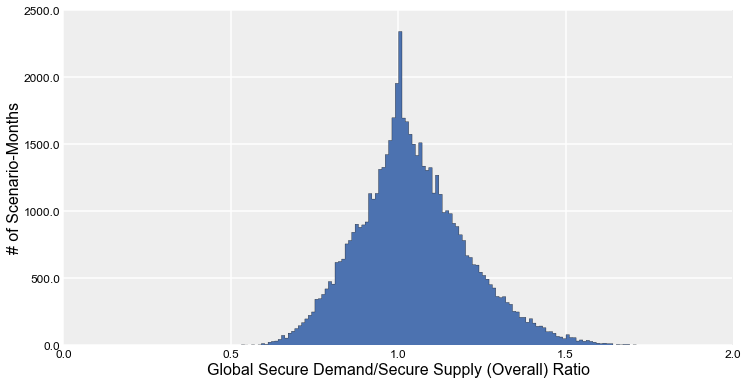
\includegraphics[width=0.75\textwidth]{Figures/OverallDistribution_lg}
	\caption{Distribution of overall ratios across all scenario-months}

\end{figure}

Figure 1 shows a histogram of the ratio between total global secure demand and supply (overall ratio) across all iteration-months. It is centered very close to 1 (a balance between supply and demand) but with a longer tail to the right; extreme supply shocks are more likely than extreme demand shocks.

\begin{figure}[h!]
	\centering
	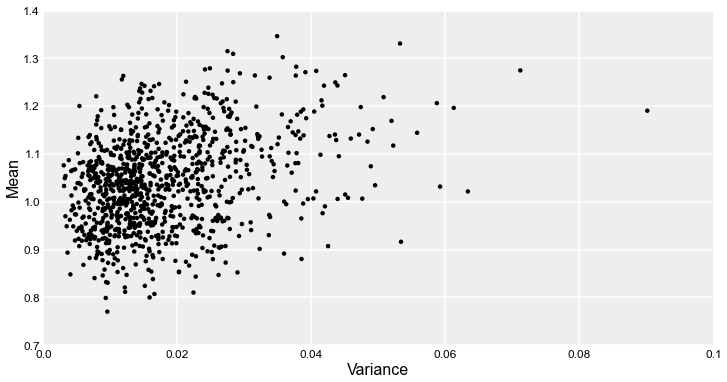
\includegraphics[width=0.75\textwidth]{Figures/OverallVarMeanScatter_lg}
	\caption{Variance and mean of overall ratio for each model iteration}
\end{figure}

I characterize each model iteration by the mean and variance of the overall ratio, as shown in Figure 2. Correlation between mean and variance is 0.33, indicating that they are not necessarily linearly related to one another. A high mean ratio may indicate higher oil insecurity, but if the variance is low, it is `stably' insecure; in contrast, the mean may be close to 1 or even below it, but high variance would indicate severe uncertainty and fluctuation -- a distinct type of insecurity. 

\subsubsection{Contagion and Assistance:}

In order to disaggregate the effects of the Contagion and Assistance model parameters, I examine their results separately. Figure 3 shows probability densities of the Overall Ratio for the scenario-months for Contagion and Assistance, respectively.

\begin{figure}[h!]
	\centering
	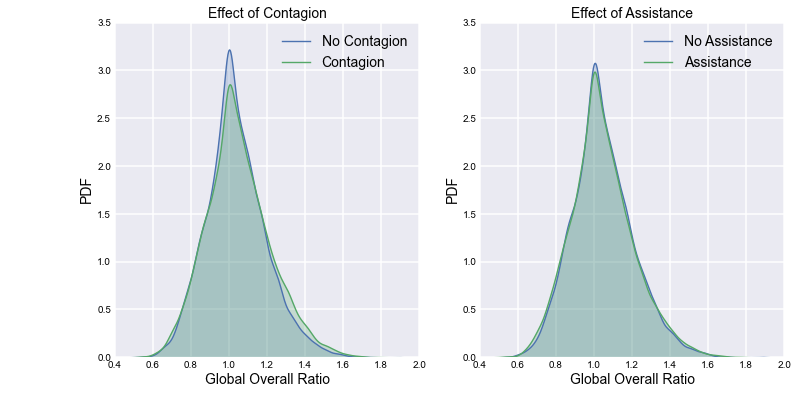
\includegraphics[width=\textwidth]{Figures/ContagionAndAssistance}
	\caption{Effects of Contagion and Assistance}
\end{figure}

The distributions with Contagion enabled and disabled appear extremely similar. I conduct several statistical tests to determine whether they are in fact drawn from the same underlying distribution, and conclude that the difference is small but statistically significant. Conflict contagion increases the mean and variance, yielding a wider range of outcomes. I repeat the same analysis for the Assistance parameter. However, in this case, the statistical tests cannot reject the hypothesis that the resulting distributions are the same, and the means are within each other's confidence intervals.

\subsection{Country-level analysis}

In addition to the aggregate global indicators, the model also tracks the Supply and Demand ratios for each country. We can analyze this output in order to understand how countries' risks differ from one another, and to identify countries at high or low risk.

\begin{figure}[h!]
	\centering
	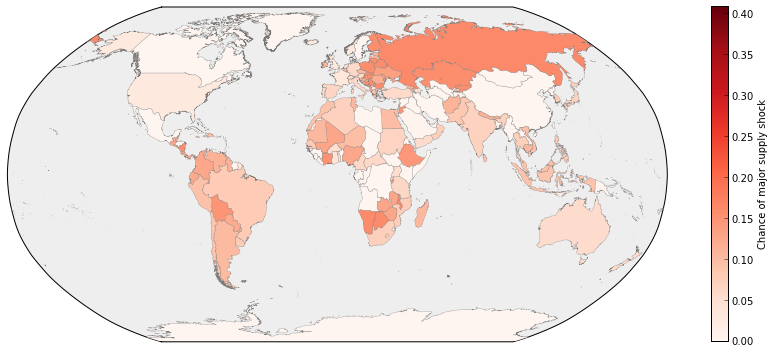
\includegraphics[width=\textwidth]{Figures/SupplyShockMap}
	\caption{Risk of a major supply shock (Supply Ratio $>2$)}

\end{figure}

Figure 4 shows a map of the overall risk of a major supply crisis, with the supply ratio rising above 2 (that is, demand exceeds secure supply by at least 100\%). Several things immediately jump out: major oil producers appear to be at the least risk, as their consumption of domestic production reduces their exposure to import disruption. Russia stands out as the one major producer to face a significant supply risk. The countries of the so-called `Global South' appears to face higher risks than the more developed world, likely indicating a lower diversity of import sources.

\begin{figure}[h!]
	\centering
	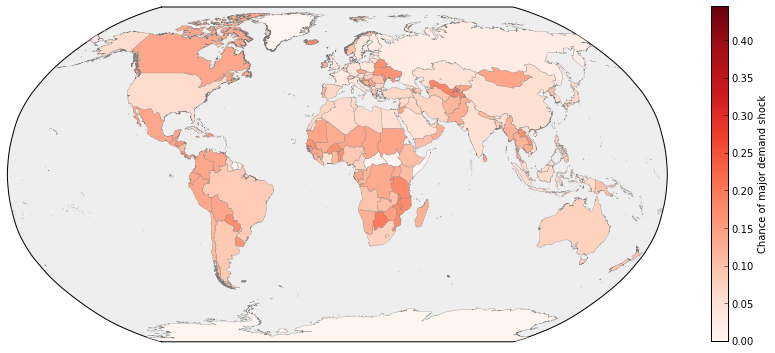
\includegraphics[width=\textwidth]{Figures/DemandShockMap}
	\caption{Risk of a major demand shock (Demand Ratio $<0.5$)}

\end{figure}

Figure 5 shows a similar map for demand risk, and indicates the likelihood of total possible exports exceeding secure exports by at least 100\%. While there are fewer countries with very low risk, there are fewer with extremely high risk as well. Interestingly, the major Middle East producers appear to face relatively low demand risk, likely indicating a robust set of trade relationships with relatively stable countries. In contrast, the major non-US producers in the Americas -- Canada, Mexico and Venezuela -- appear to face higher demand risk. This appears to be due to the fact that their exports are disproportionately to the United States, rendering them vulnerable to US crises.


\section{Discussion}

In this paper, I have described an agent-based model to study near-future international energy security, with a focus on crude oil imports and exports. The model is data-driven, ties energy security to political crises and conflicts, and can study the effects of conflict contagion and of short-term oil production increases. We can draw two sets of conclusions from the model and its outputs: on energy security itself, as well as on the challenges of modeling it, and modeling international systems more broadly.

In terms of energy security, the model does not predict extreme shocks to be likely. Nevertheless, it shows that such extreme shocks may occur within the current configuration of the international oil system, and provides an estimate for their probability. The model indicates that consumption of domestic oil production provides a significant improvement in energy security, even in the absence of total energy independence. It also highlights the importance of diverse import and export partners. The model identifies the countries facing the greatest risks to their energy security, as well as making patterns in the risk visible -- particularly the high risk in the countries of the `Global South'. 

Analysis of the Contagion and Assistance parameters yields additional interesting insight. The effect of contagion is statistically significant but small -- perhaps suggesting the difficulty facing the ongoing debate over the phenomenon in political science, but also that the debate's conclusions may not be very important to policy. More counterintuitively, perhaps, the Assistance parameter does not have a significant effect. Here is somewhere the model can generate insights that are not otherwise obvious -- specifically, that even if major oil producers can rapidly increase their output in response to crises, it is not enough to counterbalance the effects of those crises. 

From a technical perspective, the model presented here is extremely simple. The interaction between agents is minimal and largely indirect, and with both Contagion and Assistance turned off, the model is essentially stochastically sampling from the space of possible crises and durations. Nevertheless, it is sufficient to capture the core aspects of the international oil system and produces useful results, demonstrating that the approach is viable. Future work can build on this framework, adding in additional submodels, dynamics and behaviors and measuring their effect against the baseline. Such additions may include explicit oil transportation and refining accounting for systemic choke-points; allowing countries to dynamically change their trading partners, supply and demand; incorporating the risks of non-political disasters both natural (e.g. Hurricane Katrina) and manmade (such as the Deepwater Horizon spill); and more.

However, as we have seen, even the simple model presented here had extensive input requirements, with data coming from various sources of varying completeness and reliability. Expanding the model would significantly increase the data requirements. Adding dynamics and behavior pose an even greater challenge. There is no complete theory of states' energy decisionmaking -- in fact, such decisionmaking is almost certainly embedded within a broader policy framework, tied to both external interests and internal issues. It may be the case that adding additional elements will make the model more brittle without adding validity or increasing predictive power.

Finally, the model presented here may have another application, as a decision-support tool for policymakers. The model's user interface (both via input files and a graphical user interface) allows specific scenarios to be initiated and run, and their consequences and outputs evaluated. This may range from simply testing the effect of a particular events (e.g. a 12-month internal crisis in Saudi Arabia) to estimating the broader consequences of structural change (what would be the consequences if China were to become 10\% less stable, or if Iran were to begin to export to Europe). By quickly setting up and observing a `state of the world', a policymaker can augment her intuition, test hypotheses, and identify interesting issues or outliers for further qualitative or quantitative analysis. 

\bibliographystyle{splncs}
\bibliography{energysecurity}

\end{document}